\documentclass{article}
\usepackage[a4paper, total={6in, 8in}]{geometry}
\usepackage{graphicx} % Required for inserting images
\usepackage{wrapfig}    % pour les images à côté du texte
\usepackage{amssymb}
\usepackage{amsmath}
\usepackage{amsfonts}
\usepackage{extarrows}
\usepackage{soul}
\usepackage{enumitem}
\usepackage{varwidth}
\usepackage[T1]{fontenc}
\tolerance=1
\emergencystretch=\maxdimen
\hyphenpenalty=10000

\author{}
\date{}
\title{TD2: Concepts de la physique quantique}

\begin{document}
\maketitle
Dans ce TD, nous illustrons le concept de quantification de l'énergie d'un système, avec le modèle de Bohr (1913). Ce modèle (dépassé depuis 1925) permet de se familiariser avec la quantification de l'énergie, et d'expliquer simplement des phénomènes tels que les radiations lumineuses « quantifiées », c'est-à-dire selon des longueurs d'ondes fixées : à l'inverse de la lumière blanche, d'on le spectre est continu, celui d'une lampe halogène (composée d'un seul corps chimique) émet seulement selon des longueurs d'ondes bien précises, ce qui explique sa couleur, rouge pour le Néon, bleu/ultraviolet pour le Mercure, orange pour les lampes à Sodium...\newline\newline
\indent Nous abordons aussi la relation de De Broglie, qui associe une longueur d'onde à chaque particule ayant une masse, et nous illustrons le principe d'incertitude d'Heisenberg.\newline\newline

\textbf{Ex1: Modèle de Bohr(1913)}\newline
\indent L'atome d'hydrogène est constitué d'un proton de charge +q (noyau) et d'un électron de masse m et de charge -q. Le modèle de Bohr est formulé une dizaine d'années après l'idée du « quanta » émise par Planck, mais emprunte encore à la Physique classique.\newline\newline
Le modèle repose sur trois postulats :
\begin{itemize}
    \item Considérés comme ayant un mouvement circulaire uniforme de rayon r à une vitesse v, les électrons sont supposés présents sur des orbites stables, des « couches » successives correspondant chacune à un niveau d'énergie de l'électron. Ne rayonnant donc aucune énergie, l'électron ne s'«effondre» pas sur le noyau.
    \item L'électron présent sur une couche n peut passer à une couche n' en absorbant ou en émettant un photon, d'énergie fixée, quantifiée $h_{c}$, où h est la constante de Planck, c la célérité de la lumière dans le vide, et $\lambda$ la longueur d'onde du photon (Ex.2).\newline
    \item Le moment cinétique de l'électron est quantifié, ce qui se traduit par la relation suivante:
    \[
        mrv = n\frac{h}{2\pi}
        \quad
        \begin{varwidth}{\displaywidth}
            \begin{itemize}[nosep]
                \item m: masse de l'élement
                \item r: rayon de l'orbite
                \item v: vitesse de déplacement de l'électron
                \item n: numéro de la couche atomique
                \item h: constante de Planck (6,62$\times$10$^{-34}$J$\cdot$s)
            \end{itemize}
        \end{varwidth}
    \]
\end{itemize}

\begin{figure}
    \centering
    \includegraphics[scale=0.3]{rayon_orbite.png}
    \caption{Illustration de l'atome de Bohr}
\end{figure}

Le modèle de Bohr aboutit au résultat suivant : l'énergie $E_{n}$ d'un électron lié au noyau dépend de l'inverse du carré du nombre quantique n, numéro de la couche électronique où peut se trouver l'électron. C'est ce que l'on appelle la quantification des états de l'électron.
\[
    E_{n} = \frac{cste}{n^{2}}
    \quad
    \begin{varwidth}{\displaywidth}
        \begin{itemize}[nosep]
            \item n: numéro du niveau 
        \end{itemize}
    \end{varwidth}
\]
L'objectif de cet exercice est de retrouver ce résultat à partir des hypothèses de Bohr.
\begin{enumerate}
    \item En utilisant la 3e hypothèse du modèle, exprimer le produit mv en fonction de n, h et du rayon de l'orbite numéro n.\newline
    La 3ème hypothèse implique la quantification du mouvement cinétique : $\overrightarrow{L}=\overrightarrow{OM}\bigwedge\overrightarrow{p}$, avec $\overrightarrow{p}=m\overrightarrow{p}$ le vecteur quantité de mouvement\newline
    $\Longrightarrow ||\overrightarrow{L}|| = ||\overrightarrow{OM}||\times||\overrightarrow{p}||\times\sin\left(\frac{\pi}{2}\right)$=rmv\newline
    $\Longrightarrow ||\overrightarrow{L}||$ est quantifié $\rightarrow$ mrv = n$\frac{h}{2\pi}$ avec n$\in\mathbb{N^{*}}$\newline
    $\Longrightarrow$ mv = $\frac{nh}{2r\pi}$
    
    \item Rappeler l'expression de la norme de la force de Coulomb entre un électron et un proton.
    $||\overrightarrow{F_{e}}||=\frac{k|q_{1}||q_{2}|}{r^{2}}$ : force de Coulomb entre un électron et un proton (attraction)\newline
    $\Longrightarrow ||\overrightarrow{F_{e}}||=\frac{ke^{2}}{r^{2}}$; on notera $ke^{2}$={\Large e$^{2}$}
    \item Utiliser la 1ère hypothèse et le principe fondamental de la dynamique appliqué à l'électron pour exprimer le produit $mv^{2}$ en fonction de la charge élémentaire e, et du rayon r de la couche électronique.\newline
    Principe fondamental de la dynamique: $\Sigma \overrightarrow{F_{ext}} = m\overrightarrow{a}$ avec m la masse de l'électron\newline
    $\Longrightarrow ||\overrightarrow{F_{e}}|| = ma_{r}$ (le poids est négligeable devant $\overrightarrow{F_{e}}$)\newline
    $\Longrightarrow \frac{ke^{2}}{r^{2}} = m\left(\frac{v^{2}}{r}\right)$, on obtient donc:
    \[
        mv^{2} = \frac{ke^{2}}{r}
        \quad
        \begin{varwidth}{\displaywidth}
            \begin{itemize}[nosep]
                \item m: masse de l'électron (kg)
                \item e: valeur absolue de la charge de l'électron
                \item r: rayon de l'orbite
                \item k: constante de Coulomb 
            \end{itemize}
        \end{varwidth}
    \]
    \item Utiliser ces résultats pour exprimer les rayons $r_{n}$ des orbites successives accessibles à l'électron en fonction de leur nombre quantique n, c'est-à-dire le numéro de la couche électronique. Montrer qu'ils s'écrivent : $r_{n} = a_{0}n^{2}$ avec $n\in\mathbb{N}$. On appelle la constante $a_{0}$ le rayon de Bohr, qui correspond au plus petit rayon accessible.\newline
    D'après les questions précédentes, on a:
    \begin{flalign*}
        \left\{
        \begin{array}{l}
            mv = \frac{nh}{2\pi r}\\
            mv^{2} = \frac{ke^{2}}{r}    
        \end{array} & \Longrightarrow \frac{1}{m}(mv)^{2} = \frac{ke^{2}}{r} &\\
                    & \Longleftrightarrow \frac{1}{m}\left(\frac{nh}{2\pi r}\right)^{2} = \frac{ke^{2}}{r} &\\
                    & \Longleftrightarrow \frac{1}{m}\frac{n^{2}h^{2}}{4\pi^{2}r_{n}^{2}} = \frac{ke^{2}}{r_{n}} &\\
                    & \Longleftrightarrow r_{n} = \left(\frac{h^{2}}{4\pi^{2}mke^{2}}\right)n^{2}$ \text{ avec n}$\in\mathbb{N^{*}}
    \end{flalign*}
    On obtient donc
    \[
        r_{n} = \left(\frac{h^{2}}{4\pi^{2}mke^{2}}\right)n^{2}
        \quad
        \begin{varwidth}{\displaywidth}
            \begin{itemize}[nosep]
                \item $r_{n}$: rayon de l'orbite de la n-ième couche atomique
                \item h: constante de Planck (6,62$\times$10$^{-34}$J$\cdot$s)
                \item e: valeur absolue de la charge de l'électron (1,6$\times$10$^{-19}$C)
                \item m: masse de l'électron (9,1$\times$10$^{-31}$kg)
                \item k: constante de Coulomb (9$\times$10$^{-9}$SI)
            \end{itemize}
        \end{varwidth}
    \]
    On pose $a_{0}=r_{1}$ (plus petit rayon des orbites de l'électron, aussi appelé \textit{rayon de Bohr})\newline
    \underline{A.N:} $a_{0} = \frac{h^{2}}{4\pi^{2}mke^{2}} \simeq 5,29\times 10^{-11}m$
    \item Etablir, en fonction de e et du rayon $r_{n}$ d'une orbite, l'expression de l'énergie totale de l'électron $E = E_{c} + E_{pe}$ (somme de l'énergie cinétique et de l'énergie potentielle électrique $E_{pe} = \frac{k\times q_{proton}\times q_{electron}}{r}$).\newline
    \[\left\{ \begin{array}{l}
        E_{tot} = E_{c} + E_{p_{e}} \\
        E_{c} = \frac{1}{2}mv^{2} \\
        E_{p_{e}} = q_{e^{-}}\times V_{\text{tension entre $e^{-}$ et $e^{+}$}}
    \end{array}
    \Longrightarrow
    \left\{ \begin{array}{l}
        E_{p_{E}} = -\frac{ke^{2}}{r_{n}} \\
        E_{c} = \frac{1}{2}mv^{2}
    \end{array}
    \]
    Or $||\overrightarrow{F_{e}}||=\frac{mv^{2}}{r_{n}}=\frac{ke^{2}}{r_{n}^{2}}$ selon le PFD $\Longrightarrow mv^{2}=\frac{ke^{2}}{r_{n}}$\newline
    $\Longrightarrow E_{c}=\frac{1}{2}mv^{2}=\frac{1}{2}\frac{ke^{2}}{r_{n}}$\newline
    \underline{Conclusion:} $E_{tot}=-\frac{ke^{2}}{2r_{n}}$ : l'énergie est quantifiée.
    \item En déduire $E_{n}$ l'expression de l'énergie de l'électron sur l'orbite n, en fonction de e, $a_{0}$ et n. L'on pourra regrouper les constantes sous le terme $E_{1}$, énergie de la plus "basse" orbite. Quel est le nom de la constante $E_{1}$?\newline
    D'après les questions précédentes, on a:
    \[\left\{
        \begin{array}{l}
            E_{n}=-\frac{ke^{2}}{2r_{n}} = \left(-\frac{ke^{2}}{2a_{0}}\right)\frac{1}{n^{2}} = E_{1}\times\frac{1}{n^{2}} \\
            E_{1} = E(n=1): \text{énergie de l'état fondamental}
        \end{array}
    \]
    \underline{A.N:} $E_{1}=-\frac{ke^{2}}{2a_{0}} = -\frac{9\times 10^{9}\times (1,6\times 10^{-19})^{2}}{2\times 5,29\times 10^{-11}} = -2,177\times 10^{-18}J = -13,6eV$\newline
    (pour rappel: 1eV=$1,6\times$10$^{-19}$J); de la même manière on obtient
    \[E_{n}=\frac{E_{1}}{n^{2}}\left\{
        \begin{array}{l}
            n=1 \rightarrow E_{1} = -13,6eV \\
            n=2 \rightarrow E_{2} = -3,4eV \\
            n=3 \rightarrow E_{3} = -1,51eV \\
            \vdots \\
            n\to\infty \rightarrow E_{n} = 0
        \end{array}
    \]
\end{enumerate}
\newpage
\textbf{Ex2: Transitions électroniques}\newline
\indent D'après le modèle de Bohr, l'on peut calculer le diagramme d'énergie de l'électron dans l'atome d'hydrogène (voir schéma), c'est-à-dire donner les différents niveaux d'énergie de l'électron dans les différentes couches n$\in\mathbb{N^{*}}$. Remarquons que ces énergies (en électronvolts ev) sont négatives, comme vu en Ex1.\newline
(Cf figure 3 à la fin du document)

\begin{enumerate}
    \item Sur le diagramme, où se trouve le niveau d'énergie fondamental ? A quoi correspond l'état d'énergie nulle ?\newline
    Sur le diagramme, le niveau fondamental se situe au niveau n=1. L'état d'énergie nulle correspond aux états libres car n$\to$+$\infty$.
    \item Calculer la longueur d'onde du photon émis lors de la désexcitation de l'état n = 3 vers l'état n = 2. Donner le résultat en nm. La lumière émise fait-elle partie du domaine visible ? A quelle(s) série(s) appartiennent ces transitions ?\newline\newline
    Calcul de $\lambda$ du photon émis lors de la désexcitation de n=3$\to$n=2:\newline
    E3 = -1,5eV et E2 = -3,4eV donc $\frac{hc}{\lambda_{3,2}} = |\Delta E_{3,2}| = |E_{3}-E_{2}|$\newline
    $\Longrightarrow\lambda_{3,2} = \frac{hc}{|E_{2}-E_{3}|} = \frac{6,62\times 10^{-34}\times 3\times 10^{8}}{|-3,4+1,51|\times 1,6\times 10^{-19}} = 6,55\times 10^{-7}m = 655nm$ (dans le spectre du visible)\newline
    Ces transistions appartiennent au spectre de Balmer.
    \item Quelle énergie (en électronvolts puis en joules) faut-il apporter pour opérér une transition électronique de l'état fondamental vers l'état n = 3 ? Quelle est la longueur d'onde du photon permettant d'opérer cette transition ? (insérer figure 3)\newline
    $\Delta E_{1,3}=|E_{3}-E_{1}|=|-1,5+13,6|= 12,1 eV =(\text{on multiplie par } 1,6\times 10^{-19}) 1,94\times 10^{-18}J$\newline
    $\lambda_{3,1} = \frac{hc}{\Delta E_{3,1}} = \frac{6,62\times 10^{-34}\times 3\times 10^{8}}{1,94\times 10^{-18}} = 1,02\times 10^{-7}m = 102nm$ 
    \item Comment peut-on ioniser l'atome d'hydrogène depuis son état fondamental, c'est-à-dire arracher complètement l'électron à l'atome depuis l'état n = 1 ?\newline
    Lors de l'ionisation, on doit passer de n=1 à n=+$\infty$, d'après la formule: $\Delta E_{1,\infty} = E_{\infty}-E_{1}=0-(-13,6)= 13,6$eV
    \[ \lambda_{ionisation}=\frac{hc}{|E_{\infty}-E_{1}|} = \frac{hc}{|E_{1}|} = \frac{6,62\times 10^{-34}\times 3\times 10^{8}}{13,6\times 1,6\times 10^{-19}} = 91nm \]
    Pour ioniser l'atome d'hydrogène, on doit lui envoyer 13,6eV, correspondant à une longueur d'onde de 91nm.
    \newpage
    \begin{figure}[h]
        \centering
        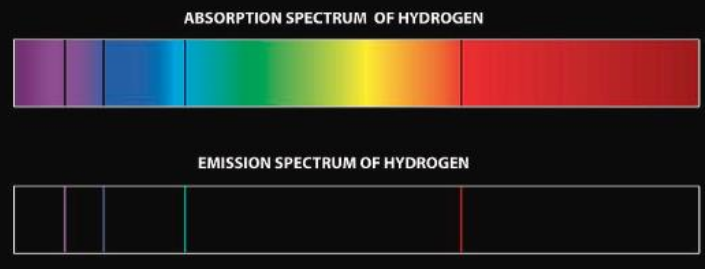
\includegraphics[scale=0.3]{figure3.png}
        \caption{Spectres d'absorption et d'émission de l'atome d'hydrogène}
    \end{figure}
    \item La Figure 2 (juste au dessus) montre les spectres d'émission et d'absorption de l'atome d'hydrogène, mesurés en laboratoire. Calculer les longueurs d'onde des transitions du tableau ci-dessous et interpréter les spectres observés.
    \begin{center}
        \begin{tabular}{|c|c|c|c|c|}
            \hline
            Transition & 3$\rightarrow$2 & 4$\rightarrow$2 & 5$\rightarrow$2 & 6$\rightarrow$2 \\
            \hline
            Longueur d'onde & 655 & 486 & 433 & 409 \\
            \hline
            Couleur & rouge-orange & bleu-vert & bleu-violet & violet \\
            \hline
        \end{tabular}
    \end{center}
    \textit{{\small Remarques : Les données du diagramme de l'hydrogène selon le modèle de Bohr peuvent être comparées à l'expérience. Pour les atomes non hydrogénoïdes et les molécules, le modèle de Bohr est insuffisant pour prévoir par le calcul l'énergie des niveaux, en raison de la présence de plusieurs électrons.}}
\end{enumerate}

\noindent\textbf{Ex3: Incertitude d'une balle de tennis : relation de De Broglie (1924) et principe d'incertitude d'Heisenberg (1927)}\newline
\indent Un électron et une balle de tennis se déplacent tous deux à une vitesse de 95 m$\cdot$s$^{-1}$, avec une incertitude sur la vitesse de 0,085\%.
\begin{enumerate}
    \item Donner la longueur d'onde de De Broglie de chacun des deux objets, considérés tous deux comme des particules.\newline
    (réponse à la question 2)
    \item Quantifier l'incertitude sur la position de l'électron et sur celle de la balle de tennis.\newline
    \begin{tabular}{|c|c|c|c|}
        \hline
         & m(kg) & $\Delta v = v\times 0,085\%$ & $\Delta x \geqslant \frac{\hbar}{2m\Delta v}$\\
        \hline
        $e^{-}$ & 9,1$\times 10^{-31}$ & 0,08m$\cdot s^{-1}$ & $\Delta x_{e^{-}}\geqslant$0,76mm\\
        \hline
        balle & 50$\times 10^{-3}$ & 0,08m$\cdot s^{-1}$ & $\Delta x_{balle}\geqslant 1,3\times 10^{-32}$m\\
        \hline
    \end{tabular}
    \item Commentaires.\newline
    Le principe n'a pas de sens à l'échelle macroscopique. Ce principe précise que si on connnait avec précision la position de la particule, alors la mesure de la vitesse de la précise (autrement, c'est toujours un compromis entre la précision de la vitesse et la précision de la position).\newline\newline
    \textbf{Données:}
    \begin{itemize}
        \item Masse d'un électron: $m_{e}=9,1\times 10^{-31}$kg
        \item Masse de la balle de tennis: m = $5,0\times 10^{-2}$kg
        \item Constante de Planck h: 6,62$\times 10^{-34} J\codt s$
    \end{itemize}
\end{enumerate}

Rappel : $mv = \frac{h}{c} = p$ pour une particule à l'échelle nanoscopique et $\lambda_{B}$: longueur d'onde de De Broglie.
\newpage
\noindent\textbf{Annexes:}\newline
\begin{figure}[h]
    \centering
    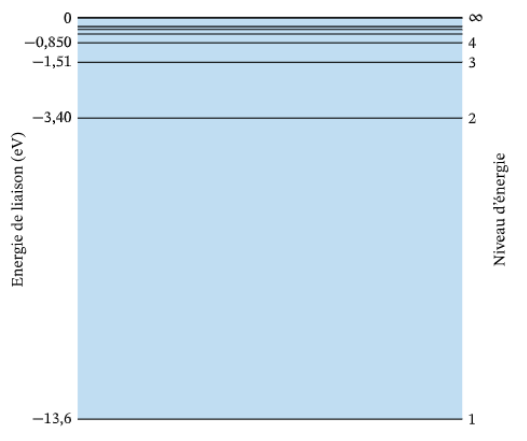
\includegraphics[scale=0.5]{figure2.png}
    \caption{Diagramme d'énergie de l'atome d'hydrogène dans le cadre du modèle de Bohr}
\end{figure}
\end{document}
